\documentclass{article}

\setlength{\headsep}{0.75 in}
\setlength{\parindent}{0 in}
\setlength{\parskip}{0.1 in}

%=====================================================
% Add PACKAGES Here (You typically would not need to):
%=====================================================

\usepackage[margin=1in]{geometry}
\usepackage{amsmath,amsthm}
\usepackage{fancyhdr}
\usepackage{enumitem}
\usepackage{graphicx}
\usepackage{float}
%=====================================================
% Ignore This Part (But Do NOT Delete It:)
%=====================================================

\theoremstyle{definition}
\newtheorem{problem}{Problem}
\newtheorem*{fun}{Fun with Algorithms}
\newtheorem*{challenge}{Challenge Yourself}
\def\fline{\rule{0.75\linewidth}{0.5pt}}
\newcommand{\finishline}{\vspace{-15pt}\begin{center}\fline\end{center}}
\newtheorem*{solution*}{Solution}
\newenvironment{solution}{\begin{solution*}}{{\finishline} \end{solution*}}
\newcommand{\grade}[1]{\hfill{\textbf{($\mathbf{#1}$ points)}}}
\newcommand{\thisdate}{\today}
\newcommand{\thissemester}{\textbf{Rutgers: Spring 2021}}
\newcommand{\thiscourse}{CS 440: Introduction to Artificial Intelligence} 
\newcommand{\thishomework}{Number} 
\newcommand{\thisname}{Name} 

\newcommand{\thisheading}{
   \noindent
   \begin{center}
   \framebox{
      \vbox{\vspace{2mm}
    \hbox to 6.28in { \textbf{\thiscourse \hfill \thissemester} }
       \vspace{4mm}
       \hbox to 6.28in { {\Large \hfill Project \#\thishomework \hfill} }
       \vspace{2mm}
         \hbox to 6.28in { { \hfill \thisdate \hfill} }
       \vspace{2mm}
       \hbox to 6.28in { \emph{Names: \thisname \hfill }}
      \vspace{2mm}}
      }
   \end{center}
   \bigskip
}

%=====================================================
% Some useful MACROS (you can define your own in the same exact way also)
%=====================================================


\newcommand{\ceil}[1]{{\left\lceil{#1}\right\rceil}}
\newcommand{\floor}[1]{{\left\lfloor{#1}\right\rfloor}}
\newcommand{\prob}[1]{\Pr\paren{#1}}
\newcommand{\expect}[1]{\Exp\bracket{#1}}
\newcommand{\var}[1]{\textnormal{Var}\bracket{#1}}
\newcommand{\set}[1]{\ensuremath{\left\{ #1 \right\}}}
\newcommand{\poly}{\mbox{\rm poly}}


%=====================================================
% Fill Out This Part With Your Own Information:
%=====================================================


\renewcommand{\thishomework}{4: Colorizing} %Homework number
\renewcommand{\thisname}{Aamna Farooq (af704), Nada Elshamaa(nhe12), and Asma Makhdoom(aam355)} % Your name
 \graphicspath{ {./images/} }

\begin{document}

\thisheading

\textbf{\Large The Basic Coloring Agent} \\
    \begin{figure}[H]
        \centering
    	\IfFileExists{images/finalBasicPic.png}{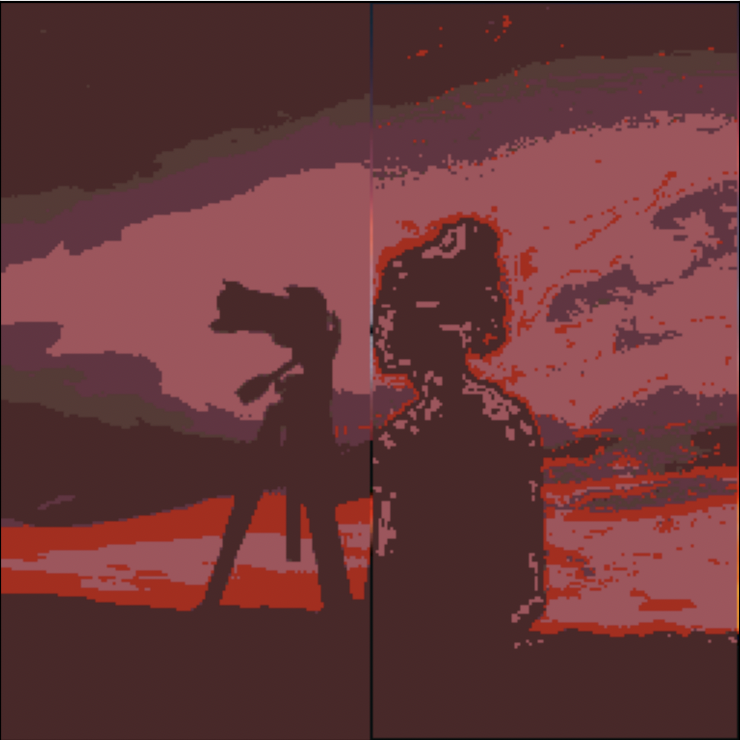
\includegraphics[]{images/finalBasicPic.png}}{No Figure Yet}
    \end{figure}
 How good is the final result? How could you measure the quality of the final result? Is it numerically satisfying, if not visually? \\
 
 The final result seems pretty impressive visually considering that it is only based off of a few representative colors. The basic agent is built by choosing 5 representative colors using Euclidean distance and k-means clustering. \\\\
 We start off by choosing 5 random points on the image and using k-means and the Euclidean distance based on color until we get more accurate 5 color points that accurately represent the colors of our data, as much as 5 colors possibly could. \\\\
 Using these 5 representative colors we recolor the left side of the image. We recolor each pixel using the color that is the smallest Euclidean distance in RGB values from a representative color. To recolor the right side of the picture we take a look at the right and left side of the gray image. We store every possible patch from the left hand side. As we go through the right side of the gray image, we get a 3x3 patch from the right side and compare it to a sample of a thousand of the left gray image's patches to find the 6 most similar patches in terms of Euclidean distance. \\\\
 Once we have located the 6 most similar patches, we use these patches to see if there is a majority recurring color in the middle pixels of these 6 patches. If there is a majority recurring color, we recolor the middle pixel of our current right patch to that color. If there is no majority then we set the color of the middle pixel of the right side to the color of the middle pixel of the most similar patch. \\\\
 The quality of the final result can be measured by comparing the Euclidean distances between the color we computed and the actual color value in the picture to get an idea of the accuracy of the program. We calculated this value to be an average of 187.02. The highest value for a euclidean distance for RGB values is 441.67 given the pixel values are as visually distinct as possible. Therefore this means that our basic algorithm performs at around 57\% similarity to the original image.\\\\
 There are abnormalities in our image, such as pixelation near the edges of figures but as per our conversation with the Professor in office hours we were reassured this is a normal irregularity and not a point of concern with our image. The image is numerically satisfying because each color is based on our Euclidean color distance formula which ensures that we are picking the closest color possible to the actual color in the image. Therefore we feel the image is numerically and visually satisfying although there is room for improvement.
  
 Bonus: Instead of doing a 5-nearest neighbor based color selection, what is the best number of representative colors to pick for your data? How did you arrive at that number? Justify yourself and be thorough. \\\\
 The best number of representative colors to pick for our data would be 10 colors. We arrived at this number through trial and error where we felt the integrity of the initial image was still preserved and that it was producing the best detailed image. With higher numbers we felt that the result was not far enough visually that it would warrant increasing the number of representative colors. 
 
 INSERT IMAGE OF 8 COLORS

\textbf{\Large The Improved Agent} \\

    \begin{figure}[H]
        \centering
    	\IfFileExists{images/finalImprovedPic.png}{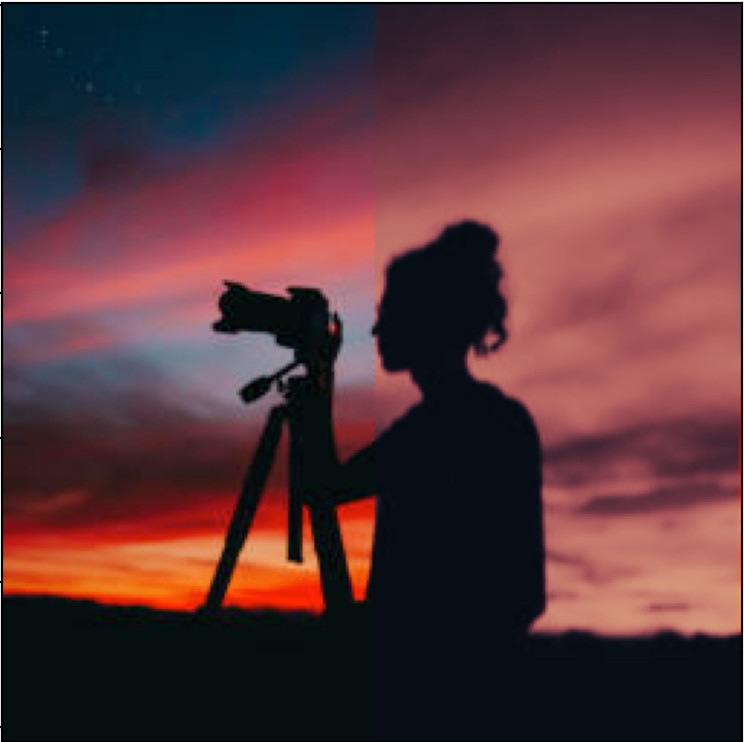
\includegraphics[]{images/finalImprovedPic.png}}{No Figure Yet}
    \end{figure}

	\textbf{Specifications}
	    Including description of input space, output space, model space, error / loss function, and learning algorithm \\
        For the improved agent we used a neural network with 3 layers in order to accomplish recoloring the image. First we convert the image into the greyscale version. Similar to the basic agent, we use the left side of the greyscale image as the training data and the right side of the greyscale image as the test data.
        The neural network is as follows: \\

        \begin{figure}[H]
            \centering
        	\IfFileExists{images/Layers.png}{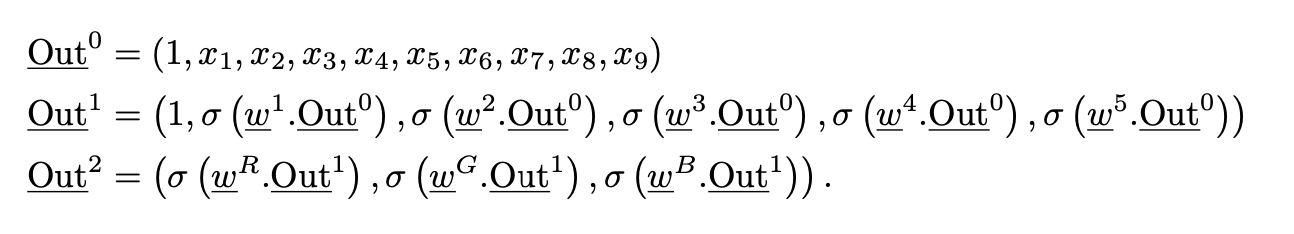
\includegraphics[width=0.8\textwidth]{images/Layers.png}}{No Figure Yet}
        \end{figure}
                
        Out1 is the input layer which is an array that holds the bias and 9 pixels from a 3x3 patch from the image, total of 10 elements. \\
        Out2 represents the hidden layer that has 6 elements and holds 50 (5*10) weights. \\
        Out3 represents the output layer and has 3 elements representing the output R, G, and B values and holds 18 (3*8) weights. \\
        
        Train the model: \\
        Initially we assign random values between 0 and 1 for the weights, which are stored in 2 separate matrices. Then we run the neural network by iterating through 3x3 patches randomly on the left hand side of the grey image starting with the random weights. Then we update the weights using stochastic gradient descent. we define the new weight value to be: \\
        
        Insert function for new weight value \\
        
        We continue to do this for 100,000 iterations keeping track of an average loss over the 100,000 patches and check to see if the loss function starts to plateau. The loss function can be defined as:\\
        
        \begin{figure}[H]
            \centering
        	\IfFileExists{images/Loss2.png}{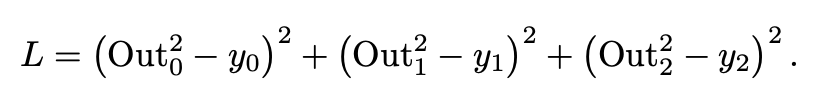
\includegraphics[width=0.5\textwidth]{images/Loss2.png}}{No Figure Yet}
        \end{figure}
        
        If the loss has decreased by less than or equal to 1\% we stop and return the new adjusted weight values. Otherwise, we continue to the next 100,000 patches until we can get to a point where the difference in loss is less than or equal to 1\%. Then we take the new computed weights to adjust the old weights. These new weights are then used to recolor the right side. In order to update the weights we had to take the partial derivative of the loss function with respect to weight which is as follows:\\
        
        \begin{figure}[H]
            \centering
        	\IfFileExists{images/Derv1.png}{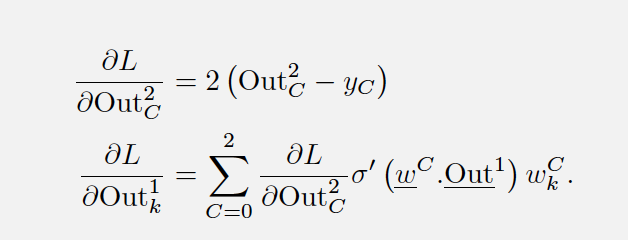
\includegraphics[width=0.6\textwidth]{images/Derv1.png}}{No Figure Yet}
        \end{figure}
        \begin{figure}[H]
            \centering
        	\IfFileExists{images/Derv2.png}{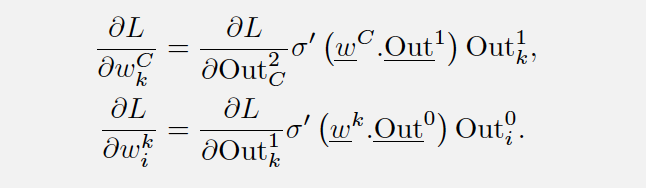
\includegraphics[width=0.6\textwidth]{images/Derv2.png}}{No Figure Yet}
        \end{figure}
        \begin{figure}[H]
            \centering
        	\IfFileExists{images/NewWeight.png}{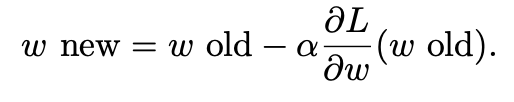
\includegraphics[width=0.45\textwidth]{images/NewWeight.png}}{No Figure Yet}
        \end{figure}
        
        Recolor Right Grey Image: \\
        In order to recolor the right side of the grey image we iterate through 3x3 patches of it and plug each patch into the neural network using the weights computed through training. This returns the output layer with a new RGB value which we use to recolor the middle pixel of the patch. We continue for all patches on the right hand side of the grey image and display the final image. \\
        
        (All equations referenced in this above portion are inspired by the Professor's Example Notes on Canvas)
        
    \\\\
    
    \textbf{Parameters}
        How did you choose the parameters (structure, weights, any decisions that needed to be made) for your model? \\\\
        Some parameters we used in the Improved Agent are alpha, having a bias for the input layer and hidden layer, iterating through 100,000 patches at a time, and choosing to stop training when the difference in loss function average changed by less than 1\%. \\\\
        We chose these parameters through suggestions from the Professor but we fine tuned them through trial and error. For example for the alpha value, we initially used a values that were very small $(10^{-10})$ and this turned out to give us unsatisfactory results. So we increased alpha until we saw significant improvements. We finalized alpha to be 0.1 initially and then it gets divided by 2 for every new patch trained on. \\\\
        Similarly, for the 1\% value, we initially started with stopping the training once the difference in loss from the previous 1000 iterations was 10\%, but this proved to be too big, so we decreased it to 5\% and then 1\% which was better for our case. \\\\
        We chose to iterate through 100,000 patches at a time in order to be able to see if the loss function was decreasing and by how much to make sure it actually plateaus. If the loss function was not decreasing after 100,000 iterations, this tells us the our weights were suitable enough to be used to color the right side of the image. \\\\
        The structure of our neural network was derived from the Professor's Example Network Notes on Canvas. This fit our use case perfectly because the input layer had nine elements which we used to represent the 9 pixels from the 3x3 patch. Also, the output layer represented RGB values which we used to recolor the middle pixel from the input patch. We chose to update our weights and to calculate the derivative of the loss functions with respect to weights using these notes.
        
    \textbf{Pre-processing}
        Any pre-processing of the input of output data that you used.
        \begin{solution} \hfill \\
        
        We pre-processed the input data by normalizing all the RGB values to be between 0 and 1 instead of between 0 and 255. This was important so that the value of alpha would not need to be too inflated and we would be able to reach a desirable result earlier. This was also important in ensuring the output values of the color were more distinct from one another and to ensure the RGB values were not close to one another.\\\\
        We also pre-processed the data by converting the image into gray-scale using the equation provided: \\\\
        Gray(r, g, b) = 0.21r + 0.72g + 0.07b \\\\
        so that we could train the data using the gray-scale of the image. \\\\
        We also split the image into two halves so that we can use the left side of the image to train our weights using the neural network. We then use the right side of the image to recolor the image using the weights we finalized from the training of the data. 
        \end{solution}\\\\
        
    \textbf{Training}
        How did you handle training your model? How did you avoid overfitting? 
        \begin{solution} \hfill \\
        We start off the training by assigning random values between 0 and 1 for the weights. Then we train the neural network to produce more accurate weights using the left side of the grey image. We do this by storing all the patches from the left side of the grey image into an array. Then we pick a patch randomly from the array and plug it into the neural network as the input layer to calculate the hidden layer and output layer. Using the newly calculated output layer we calculate the loss function in order to compare to computed output to the expected output and store this value. Then we update the weights using stochastic gradient descent and repeat this on a set of 100,000 patches, keeping track of an avg loss each iteration. Once we reach 100,000 patches we compare the avg loss to the avg loss of the previous 100,000 set of patches. If the difference between the losses is greater than .01\% we continue to the next 100,000 set of patches. Otherwise if it is less than or equal to .01\% we immediately return the weights for the output and hidden layers because this is the most accurate weights based on the training data.\\\\
        In order to avoid overfitting we made sure to try out our algorithm using different combinations of averages and alpha values. Initially we were only comparing the loss from the previous 1000 set of patches to the loss after those 1000 patches without calculating a running average of the patching. This proved to produce weights that were not accurate and as a result our resulting was very washed out and white. After some trial and error, we settled with using an average of loss over 100,000 patches and this seemed to work best with our input image. Similarly, for alpha, through trial and error, we chose the value to be 0.1 initially and for every step in gets divided by 2. This proved to give us the best results.
        \end{solution}\\\\
        
    \textbf{Evaluation}
        An evaluation of the quality of your model compared to the basic agent. How can you quantify and qualify the differences between their performance? How can you make sure that the comparison is 'fair'? 
        \begin{solution} \hfill \\
        Compared to the basic agent, the improved agent performs really well. Visually you can see that the improved agent returns a much better quality photo compared to the pixely basic agent result.\\\\
        The quantify and qualify this, the quality of the final result can be measured by comparing the Euclidean distances between the color we computed and the actual color value in the picture to get an idea of the accuracy of the program. We calculated this value to be an average of 98.50 for the improved agent and 187.02 for the basic agent. Already we see that the average distance for the improved agent is smaller than the basic agent, meaning it is closer to the original image compared to the basic agent. \\\\
        The highest value for a euclidean distance for RGB values is 441.67 given the pixel values are as visually distinct as possible. Therefore this means that our improved agent performs at 77.7\% and the basic agent performs at around 57\% which is a big improvement.\\\\
    
        \end{solution}\\\\
        
    \textbf{Improvements}
        How might you improve your model with sufficient time, energy, and resources?
        \begin{solution} \hfill \\
    
        \end{solution}\\\\
\smallskip

\textbf{\Large Bonus} \\
    Why is a linear model a bad idea? 
    \begin{solution} \hfill \\
    
    \end{solution}\\
    
    Research a ML framework like scikit-learn or tensorflow, and build a solution to this problem using this framework that beats your improved agent.
    \begin{solution} \hfill \\
    
    \end{solution}\\

\smallskip   

\textbf{Work Distribution}
\\
The work is our own and not copied or taken from any other students. 
\\\\
To work on this project we would meet up over video calls daily and discuss problems and our solutions. One person would then screen share and code while the others would contribute and also assist in coding using the request remote control feature in zoom. We would alternate in screen sharing and upload to git for version control. 
\\\\
The report was done similarly. We each took on a plot and a question to complete on our own. We then met to complete the rest as a group over video call. 
\\
$Asma$ $Makhdoom:$ 
\\
$Aamna$ $Farooq:$ 
\\
$Nada$ $Elshamaa:$ 
\\
\smallskip

\end{document}